\documentclass[letterpaper, 12pt]{article}
\usepackage[american]{babel}
\usepackage[utf8]{inputenc}
\usepackage[citestyle=apa,style=apa,backend=biber]{biblatex}
\usepackage[margin=1in]{geometry}
\usepackage{graphicx}
\usepackage{caption}
\usepackage{float}
\setlength\bibitemsep{2\itemsep}
\DeclareLanguageMapping{american}{american-apa}
\addbibresource{bibliography.bib}

\pagenumbering{roman}

\begin{document}
\begin{titlepage}
\centering
	\vspace*{5.75cm}
	{\huge\bfseries A literature review of Internet of Things security\par}
	\vspace{2cm}
	Blair Urish\\
	Kansas State University\\
	College of Engineering\\
	Department of Computer Science\\
	\vspace{1cm}
	Dr. William Hsu\\
	Professor\\
	Department of Computer Science\\
	\vspace{1cm}
	May 2017
\end{titlepage}


\begin{abstract}
\thispagestyle{plain}
\setcounter{page}{2}
\begin{flushleft}
	Lorem ipsum dolor sit amet, consectetur adipiscing elit, sed do 
eiusmod tempor incididunt ut labore et dolore magna aliqua. Ut 
enim ad minim veniam, quis nostrud exercitation ullamco. 
Lorem ipsum dolor sit amet, consectetur adipiscing elit, sed do 
eiusmod tempor incididunt ut labore et dolore magna aliqua. Ut 
enim ad minim veniam, quis nostrud exercitation ullamco laboris
Lorem ipsum dolor sit amet, consectetur adipiscing elit, sed do 
eiusmod tempor incididunt ut labore et dolore magna aliqua. Ut 
enim ad minim veniam, quis nostrud exercitation ullamco laboris
\end{flushleft}
\end{abstract}

\newpage
\setcounter{page}{3}
\tableofcontents
\newpage

\cleardoublepage
\addcontentsline{toc}{section}{\listfigurename}
\listoffigures
\newpage

\pagenumbering{arabic}
\begin{flushleft}
\section*{Introduction}
\addcontentsline{toc}{section}{Introduction}
This section will discuss background information related to the report's topic. The section will contain the historical background of the issue, a brief
overview of the current research, and discuss the purpose of this research. \\
~\newline
\textit{Historical Background}\\ 
~\newline
By 2020, it is expected that there will be 
25 million Internet of Things devices connected to the Internet. (\cite{Martinez1}). With so many devices, it is important that manufacturers take security very seriously. 
In September 2016, a security researcher named Brian Krebs had his website temporarily taken down due to a Distributed Denial of Service attack. The attacker
used thousands of malware-infected IoT devices and sent 600 Gigabits per second of traffic to Krebs' blog. (\cite{Krebs}). The malware, called Mirai, 
infected IoT devices with poor security. An analysis showed that the devices were mainly CCTV cameras, DVRs, and routers. (\cite{Incapsula}).\\
~\newline
A few months later, in December 2016, SEC Consult discovered a backdoor in Sony IPELA Engine IP Cameras that allowed for full remote access over the Internet. (\cite{sec}). The backdoor could allow an attacker
to install malicious code on the device. At the time of the disclosure, there were at least 4,250 devices at risk. (\cite{Krebs2}). Owners of the affected devices must manually update them
to be safe from potential attack. No malware has targeted these devices yet, but it is possible that may change in the future if the owners do not update their devices. Overall, these two incidents
are just a few examples of the problems with IoT security.\\
~\newline
\textit{Overview of Current Research}\\
~\newline
The literature outlines security risks in all layers of the Internet of Things architecture. (\cite{Xiaohui6643029}; \cite{Zhao6746513}; \cite{Suo6188257}). 
There is some debate as to which layers need the most attention for future research. Some argue that risks in the perception layer present the greatest risk. (\cite{Zhao6746513}).
Others argue that security at the perception layer is of a lower priority. (\cite{Kozlov}). \\
~\newline
As for security standards, the Constrained Application Protocol suggests the use of Datagram Transport Layer Security (DTLS). However, this introduces a large amount of overhead. (\cite{Capossele}).  
Other literature has considered the use of the Host Identity Protocol (HIP) instead. (\cite{Garcia-Morchon:2013:SII:2462096.2462117}). The literature found that HIP has less overhead when compared to
DTLS. Some literature has even proposed extensions to HIP that would further reduce overhead (\cite{Hummen}).\\
~\newline
\textit{Purpose of the Research}\\
~\newline
The purpose of this literature review is to synthesize the existing research regarding the security risks, standards, and government action into one report. There are many different points of view in the
literature about which areas of the IoT are most at risk. There is also conflict in the literature regarding which standards should be used and how they should be implemented. With this literature review,
all of this debate will be collected into one report which will make it easier for future research to be done. \\
~\newline
\textit{Structure of Report}\\
~\newline
The report will first cover the methods used to gather the relevant research. Next, the report will discuss the security risks for current IoT devices. Then, the report will synthesize the research being
done to develop new security standards and protocols. The report will then discuss current and future government standards for IoT security. Finally, the findings of the report will be summarized in the conclusion
section.

\section*{Methodology}
\addcontentsline{toc}{section}{Methodology}

To create the report, information from academic journals and conference proceedings were used. These articles were found in 
databases such as Scopus, IEEE, and the ACM. Search terms such as "Internet of Things" and "security" were used to locate
relevant articles in the databases. Web sources from industry leaders were used to provide background information surrounding
the topic.\\ 


\section*{Security Risks for IoT Devices}
\addcontentsline{toc}{section}{Security Risks for IoT Devices}

This section will discuss the security risks faced by current IoT devices. The section will use the three main layers of the IoT architecture to break down the risks. Before the risks at each layer are discussed,
the IoT architecture will be formally defined. After that the risks found in the perception layer, network layer, and application layer will be discussed.

\subsection*{Defining the IoT Architecture}
\addcontentsline{toc}{subsection}{Defining the IoT Architecture}
The literature generally breaks the IoT architecture down into three layers: perception, network, and application. (\cite{Zhao6746513}; \cite{Xiaohui6643029}). Some literature adds additional layers to further narrow down the purpose of each
layer. (\cite{Granjal7005393}; \cite{Kozlov}; \cite{Suo6188257}). However, for the purposes of this report, three layers will be sufficient. The perception layer 
generally includes the devices that allow an IoT device to interact with the physical world. A temperature sensor would be an example of a
perception layer device. The network layer includes devices that allow the perception layer and application layer to interact through the Internet.
Traditional network hardware is included in this layer. Finally, the application layer is defined as the software that allows end users to control
and retrieve data from the perception layer devices. Below is a figure that gives more examples of devices that are commonly found at each layer.

\begin{figure}[H]
	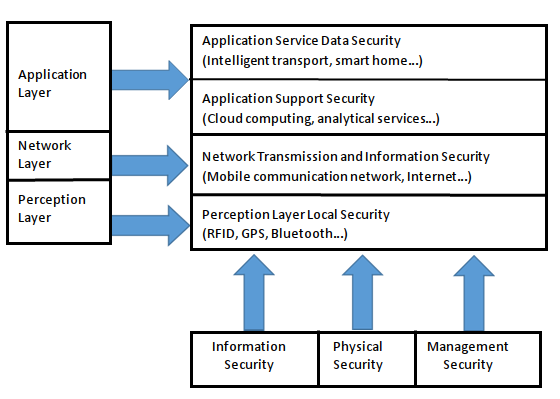
\includegraphics[width=\linewidth,height=10cm,keepaspectratio]{figure2_new.png}
	\caption{Internet of Things Architecture (adapted from \cite{Zhao6746513})}
	\label{fig:arch}
\end{figure}

\subsection*{Security Risks in the Perception Layer}
\addcontentsline{toc}{subsection}{Security Risks in the Perception Layer}
In the perception layer, devices are commonly found in public with minimal physical security. The literature states that there is a risk of an attacker physically
modifying a device at this layer. (\cite{Zhao6746513}; \cite{Xiaohui6643029}; \cite{Suo6188257}). Devices in the perception layer, for the most part,
are not very powerful. The devices use processors that prioritize efficiency and cost over speed. Due to this limitation, they are often unable to use the same security mechanisms found in traditional computers. 
(\cite{Suo6188257}; \cite{Granjal7005393}; \cite{Xiaohui6643029}). Even traditional attack methods used to target conventional computers could be 
used against the IoT. (\cite{Zhao6746513}). Attacks such as distributed denial of service (DDoS) could disrupt sensors from communicating with the devices that receive the gathered information. Devices in the perception layer are also suceptible to malware, as shown by the recent Mirai
botnet which infected thousands of IoT devices. (\cite{Incapsula}). 

\subsection*{Security Risks in the Network Layer}
\addcontentsline{toc}{subsection}{Security Risks in the Network Layer}
Many of the security risks in the network layer are already well-known, because they also apply to traditional computing platforms. 
(\cite{Zhao6746513}; \cite{Xiaohui6643029}). According to Zhao and Ge, the security implementations found in the network layer are fairly complete, but
the risks should not be ignored. The most common threats found in the network layer include man-in-the-middle attacks, illegal access due to 
insufficient authentication measures, information eavesdropping, and many others. These types of attacks put the privacy of users at risk as most
information transmitted is from the physical world. 

\subsection*{Security Risks in the Application Layer}
\addcontentsline{toc}{subsection}{Security Risks in the Application Layer}
Like the network layer, many of the security risks present in the layer are also found on traditional computing platforms. The literature outlines
risks such as software vulnerabilities and insecure authentication methods. (\cite{Zhao6746513}; \cite{Suo6188257}). Just like with traditional
platforms, mistakes by programmers that introduce vulnerabilities like buffer overflow are still common with IoT software. For authentication,
the developers must ensure that users are only allowed to access data they need. IoT devices commonly collect sensitive information that could
violate the privacy of the public if it got into the wrong hands. (\cite{Zhang:2015:EST:2714576.2737091}). 

\section*{IoT Security Protocol Standardization}
\addcontentsline{toc}{section}{IoT Security Protocol Standardization}

This section will first outline the need for a standardized suite of protocols to ensure security for the IoT. It will then evaluate various protocols
that have been proposed and outline any debate found in the literature. The protocols that will be discussed include the Constrained Application
Protocol (CoAP), IEEE 802.15.4, 6LoWPAN, Datagram Transport Layer Security (DTLS), and the Host Identity Protocol (HIP). 

\subsection*{The Need for Standardization}
\addcontentsline{toc}{subsection}{The Need for Standardization}
Many of the protocols required to ensure security for the IoT already exist but most IoT devices are not powerful enough to use them. (\cite{Keoh6817545}; \cite{Granjal7005393}; \cite{Garcia-Morchon:2013:SII:2462096.2462117}). Currently, standardization efforts are underway by the
Institute for Electrical and Electronics Engineers (IEEE) and the Internet Engineering Task Force (IETF). One project by the IETF is the
Constrained Application Protocol (CoAP). CoAP is a protocol similar to HTTP that allows devices to make requests and receive responses. (\cite{Keoh6817545}). The most commonly used protocol used to secure CoAP is Datagram Transport Layer Security (DTLS). (\cite{Keoh6817545}; \cite{Garcia-Morchon:2013:SII:2462096.2462117}). 
Some literature proposes the use of the Host Identity Protocol (HIP) as an alternative to DTLS. (\cite{Hummen}; \cite{Garcia-Morchon:2013:SII:2462096.2462117};). The conflict in the literature on this issue alone shows the need for standardization. As pointed out by Koeh et. al, the reason for the success of the HyperText Transfer Protocol (HTTP) has been the completely standardized protocol suite. For the Internet
of Things to have a successful and secure future, the industry must agree on a standardized security suite.

\subsection*{The Constrained Application Protocol}
\addcontentsline{toc}{subsection}{The Constrained Application Protocol}


\subsection*{Datagram Transport Layer Security}
\addcontentsline{toc}{subsection}{Datagram Transport Layer Security}
This section will begin by discussing the findings of Garcia-Morchon et. al. regarding the viability of Datagram Transport Layer security (DTLS)
for securing CoAP messages. To start with, DTLS is simply TLS over the UDP protocol instead of TCP. The CoAP recommends using DTLS in place of any
other method. However, one major issue with DTLS is that it is designed for traditional networks. (\cite{Capossele}). In the Garcia-Morchon et. al. report, the authors analyzed the performance of DTLS using a custom application running on a Redbee Econotag. The device
was used to simulate a real world IoT device. The authors found that DTLS used a significant amount of memory due to the amount of messages sent. 
The authors also found that DTLS does not perform well in a network with high packet loss. \\
~\newline
The work of Garcia-Morchon et. al. demonstrates the need for additional changes to enable DTLS to work with the IoT. Capossele, Cervo, De Cicco,
and Petrioli released a report outlining their optimized DTLS implementation. For their work, they used a MagoNode to simulate the presence of an
IoT device. The specifications of the test device were similar to the one used by Garcia-Morchon et. al., but with 16 KB of RAM instead of 128 KB.
In order to make DTLS functional on their test device, the authors optimized modular arithmetic on large integers using their own assembly code.
The authors also created their own ECC library to further optimize the cryptographic functions. The authors analyzed the results by separating their
optimizations in order to see which ones had the greatest impact on performance. In the table below, one can see which optimization was performed,
the time the operation took, the energy used, and the increase in ROM usage. 

\begin{figure}[H]
	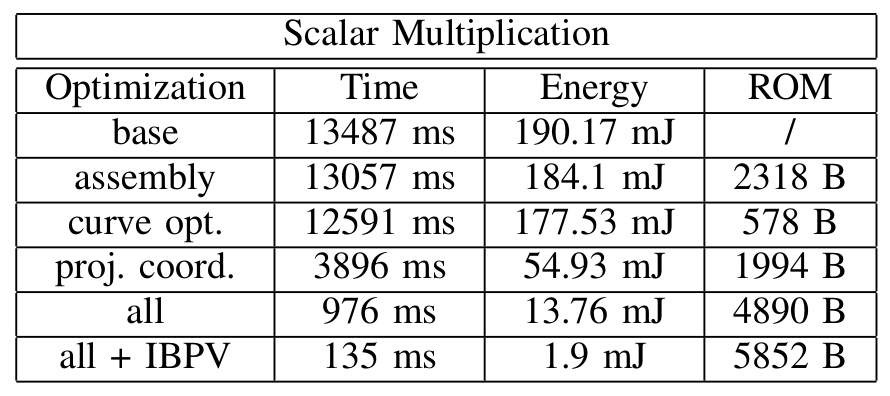
\includegraphics[width=\linewidth,height=7cm,keepaspectratio]{figure6.png}
	\caption{Scalar Multiplication Time Comparison (\cite{Capossele})}
	\label{fig:arch}
\end{figure}

As one can see from the figure, the optimizations together provide a large increase in performance, but at the expense of more ROM usage. 

\newpage
\addcontentsline{toc}{section}{References}
\printbibliography
\end{flushleft}
\end{document}
